\documentclass[tikz,border=5pt]{standalone}

\usetikzlibrary{calc, intersections}
\usepackage{xfp}
\usepackage{mathrsfs} % Add macro \mathscr which is used for labeling circles.

\begin{document}
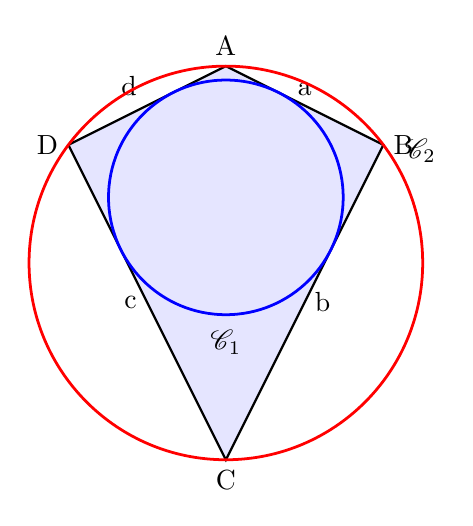
\begin{tikzpicture}

% Cuadrilátero bicéntrico pequeño.
\coordinate (A) at (0, 1);
\coordinate (B) at (2, 0);
\coordinate (C) at (0, -4);
\coordinate (D) at (-2, 0);

% Cuadrilátero bicéntrico mediano.
%% \coordinate (A) at (0, 2);
%% \coordinate (B) at (4, 0);
%% \coordinate (C) at (0, -8);
%% \coordinate (D) at (-4, 0);

% Cuadrilátero bicéntrico grande.
%% \coordinate (A) at (0, 4);
%% \coordinate (B) at (8, 0);
%% \coordinate (C) at (0, -16);
%% \coordinate (D) at (-8, 0);

\path let \p1=(A), \p2=(B), \p3=(C), \p4=(D)
    in node[draw=none] at (0,0) {
        % Compute side lengths
        \xdef\sideAB{\fpeval{sqrt((\x2-\x1)^2 + (\y2-\y1)^2)}}
        \xdef\sideBC{\fpeval{sqrt((\x3-\x2)^2 + (\y3-\y2)^2)}}
        \xdef\sideCD{\fpeval{sqrt((\x4-\x3)^2 + (\y4-\y3)^2)}}
        \xdef\sideDA{\fpeval{sqrt((\x1-\x4)^2 + (\y1-\y4)^2)}}
        % Compute diagonal lengths
        \xdef\diagAC{\fpeval{sqrt((\x3-\x1)^2 + (\y3-\y1)^2)}}
        \xdef\diagBD{\fpeval{sqrt((\x4-\x2)^2 + (\y4-\y2)^2)}}
    };

\edef\isTangential{\fpeval{abs((\sideAB + \sideCD) - (\sideBC + \sideDA)) < 0.001 ? 1 : 0}}
\edef\isCyclic{\fpeval{abs(\diagAC*\diagBD - (\sideAB*\sideCD + \sideBC*\sideDA)) < 0.001 ? 1 : 0}}

\ifnum\isTangential=1
   \ifnum\isCyclic=1
        %% Draw quadrilateral and labels

        \draw[fill=blue!10!white, thick]
                 (A) node[above]{A}
              -- node [above]{a} (B) node[right]{B}
              -- node [right]{b} (C) node[below]{C}
              -- node [left]{c} (D) node[left]{D}
              -- node [above left]{d} cycle;

        %% Draw incircle

        \coordinate(G1) at ($(A)!1cm!(B)$);
        \coordinate(G2) at ($(A)!1cm!(D)$);
        \coordinate(M1) at ($(G1)!.5!(G2)$);
        \path[name path=angleBisector1]
            let \p1=(A), \p2=(C), \n1={veclen(\y2-\y1,\x2-\x1)}
            in (A) -- ($(A)!\n1!(M1)$);

        \coordinate(H1) at ($(B)!1cm!(A)$);
        \coordinate(H2) at ($(B)!1cm!(C)$);
        \coordinate(M2) at ($(H1)!.5!(H2)$);
        \path[name path=angleBisector2]
            let \p1=(B), \p2=(D), \n1={veclen(\y2-\y1,\x2-\x1)}
            in (B) -- ($(B)!\n1!(M2)$);

        \draw [blue, line width = 1pt, name intersections={of=angleBisector1 and angleBisector2, by={centerOfIncircle}}]
            let \p1=(centerOfIncircle), \p2=($(A)!(centerOfIncircle)!(B)$), \n1={veclen(\y2-\y1,\x2-\x1)}
            in (centerOfIncircle) circle [red, radius=\n1]
            \pgfextra{\xdef\radiusOfIncircle{\n1}};

         %% Draw circumcircle

         \coordinate (M1) at ($(A)!0.5!(B)$);
         \path[name path=bisectorAB, overlay] ($(M1)!10!-90:(B)$) -- ($(M1)!10!90:(B)$);

         \coordinate (M2) at ($(B)!0.5!(C)$);
         \path[name path=bisectorBC, overlay] ($(M2)!10!90:(C)$) -- ($(M2)!10!-90:(C)$);

         \draw [red, line width = 1pt, name intersections={of=bisectorAB and bisectorBC, by={centerOfCircumcircle}}]
             let \p1=(centerOfCircumcircle), \p2=(A), \n1={veclen(\y2-\y1,\x2-\x1)}
             in (centerOfCircumcircle) circle [radius=\n1]
            \pgfextra{\xdef\radiusOfCircumcircle{\n1}};

         % Show labels for incircle and circumcircle
         \def\offset{10}
         \def\incircleAngleLabel{270}
         \def\circumcircleAngleLabel{30}
         \draw node at ($(centerOfIncircle) + (\incircleAngleLabel:\radiusOfIncircle + \offset)$) {$\mathscr{C}_1$};
         \draw node at ($(centerOfCircumcircle) + (\circumcircleAngleLabel:\radiusOfCircumcircle + \offset)$) {$\mathscr{C}_2$};

    \else
        \node[red, font=\bfseries] at (0,0) {This quadrilateral is tangential, but is not cyclic.};
    \fi
\else
    \node[red, font=\bfseries] at (0,0) {This quadrilateral is not tangential.};
\fi
\end{tikzpicture}
\end{document}
